% Made up for the tikra benchmark.
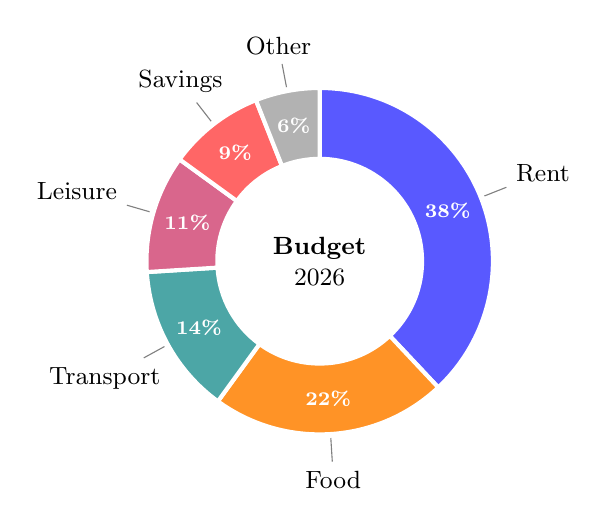
\begin{tikzpicture}[font=\small]
  \def\ro{2.2} \def\ri{1.3}
  \def\angle{90}
  \foreach \pct/\col/\name in {38/blue!65/Rent, 22/orange!85/Food, 14/teal!70/Transport,
      11/purple!60/Leisure, 9/red!60/Savings, 6/gray!60/Other} {
    \pgfmathsetmacro\sweep{3.6*\pct}
    \pgfmathsetmacro\stop{\angle-\sweep}
    \pgfmathsetmacro\mid{\angle-\sweep/2}\pgfmathsetmacro\opp{\mid+180}
    \fill[\col, draw=white, line width=1.5pt] (\angle:\ro) arc[start angle=\angle, end angle=\stop, radius=\ro]
      -- (\stop:\ri) arc[start angle=\stop, end angle=\angle, radius=\ri] -- cycle;
    \node[white, font=\scriptsize\bfseries] at (\mid:{(\ro+\ri)/2}) {\pct\%};
    \draw[gray] (\mid:\ro+0.05) -- (\mid:\ro+0.35) node[anchor=\opp, black] {\name};
    \global\let\angle\stop
  }
  \node[align=center] at (0,0) {\textbf{Budget}\\ 2026};
\end{tikzpicture}
